% GNUPLOT: LaTeX picture with Postscript
\begingroup
  \makeatletter
  \providecommand\color[2][]{%
    \GenericError{(gnuplot) \space\space\space\@spaces}{%
      Package color not loaded in conjunction with
      terminal option `colourtext'%
    }{See the gnuplot documentation for explanation.%
    }{Either use 'blacktext' in gnuplot or load the package
      color.sty in LaTeX.}%
    \renewcommand\color[2][]{}%
  }%
  \providecommand\includegraphics[2][]{%
    \GenericError{(gnuplot) \space\space\space\@spaces}{%
      Package graphicx or graphics not loaded%
    }{See the gnuplot documentation for explanation.%
    }{The gnuplot epslatex terminal needs graphicx.sty or graphics.sty.}%
    \renewcommand\includegraphics[2][]{}%
  }%
  \providecommand\rotatebox[2]{#2}%
  \@ifundefined{ifGPcolor}{%
    \newif\ifGPcolor
    \GPcolorfalse
  }{}%
  \@ifundefined{ifGPblacktext}{%
    \newif\ifGPblacktext
    \GPblacktexttrue
  }{}%
  % define a \g@addto@macro without @ in the name:
  \let\gplgaddtomacro\g@addto@macro
  % define empty templates for all commands taking text:
  \gdef\gplbacktext{}%
  \gdef\gplfronttext{}%
  \makeatother
  \ifGPblacktext
    % no textcolor at all
    \def\colorrgb#1{}%
    \def\colorgray#1{}%
  \else
    % gray or color?
    \ifGPcolor
      \def\colorrgb#1{\color[rgb]{#1}}%
      \def\colorgray#1{\color[gray]{#1}}%
      \expandafter\def\csname LTw\endcsname{\color{white}}%
      \expandafter\def\csname LTb\endcsname{\color{black}}%
      \expandafter\def\csname LTa\endcsname{\color{black}}%
      \expandafter\def\csname LT0\endcsname{\color[rgb]{1,0,0}}%
      \expandafter\def\csname LT1\endcsname{\color[rgb]{0,1,0}}%
      \expandafter\def\csname LT2\endcsname{\color[rgb]{0,0,1}}%
      \expandafter\def\csname LT3\endcsname{\color[rgb]{1,0,1}}%
      \expandafter\def\csname LT4\endcsname{\color[rgb]{0,1,1}}%
      \expandafter\def\csname LT5\endcsname{\color[rgb]{1,1,0}}%
      \expandafter\def\csname LT6\endcsname{\color[rgb]{0,0,0}}%
      \expandafter\def\csname LT7\endcsname{\color[rgb]{1,0.3,0}}%
      \expandafter\def\csname LT8\endcsname{\color[rgb]{0.5,0.5,0.5}}%
    \else
      % gray
      \def\colorrgb#1{\color{black}}%
      \def\colorgray#1{\color[gray]{#1}}%
      \expandafter\def\csname LTw\endcsname{\color{white}}%
      \expandafter\def\csname LTb\endcsname{\color{black}}%
      \expandafter\def\csname LTa\endcsname{\color{black}}%
      \expandafter\def\csname LT0\endcsname{\color{black}}%
      \expandafter\def\csname LT1\endcsname{\color{black}}%
      \expandafter\def\csname LT2\endcsname{\color{black}}%
      \expandafter\def\csname LT3\endcsname{\color{black}}%
      \expandafter\def\csname LT4\endcsname{\color{black}}%
      \expandafter\def\csname LT5\endcsname{\color{black}}%
      \expandafter\def\csname LT6\endcsname{\color{black}}%
      \expandafter\def\csname LT7\endcsname{\color{black}}%
      \expandafter\def\csname LT8\endcsname{\color{black}}%
    \fi
  \fi
  \setlength{\unitlength}{0.0500bp}%
  \begin{picture}(12960.00,10080.00)%
    \gplgaddtomacro\gplbacktext{%
      \csname LTb\endcsname%
      \put(1078,704){\makebox(0,0)[r]{\strut{} 0}}%
      \csname LTb\endcsname%
      \put(1078,2156){\makebox(0,0)[r]{\strut{} 50}}%
      \csname LTb\endcsname%
      \put(1078,3609){\makebox(0,0)[r]{\strut{} 100}}%
      \csname LTb\endcsname%
      \put(1078,5061){\makebox(0,0)[r]{\strut{} 150}}%
      \csname LTb\endcsname%
      \put(1078,6513){\makebox(0,0)[r]{\strut{} 200}}%
      \csname LTb\endcsname%
      \put(1078,7966){\makebox(0,0)[r]{\strut{} 250}}%
      \csname LTb\endcsname%
      \put(1078,9418){\makebox(0,0)[r]{\strut{} 300}}%
      \csname LTb\endcsname%
      \put(1210,484){\makebox(0,0){\strut{} 0}}%
      \csname LTb\endcsname%
      \put(2944,484){\makebox(0,0){\strut{} 5}}%
      \csname LTb\endcsname%
      \put(4679,484){\makebox(0,0){\strut{} 10}}%
      \csname LTb\endcsname%
      \put(6413,484){\makebox(0,0){\strut{} 15}}%
      \csname LTb\endcsname%
      \put(8147,484){\makebox(0,0){\strut{} 20}}%
      \csname LTb\endcsname%
      \put(9882,484){\makebox(0,0){\strut{} 25}}%
      \csname LTb\endcsname%
      \put(11616,484){\makebox(0,0){\strut{} 30}}%
      \put(11748,704){\makebox(0,0)[l]{\strut{} 0}}%
      \put(11748,2156){\makebox(0,0)[l]{\strut{} 50}}%
      \put(11748,3609){\makebox(0,0)[l]{\strut{} 100}}%
      \put(11748,5061){\makebox(0,0)[l]{\strut{} 150}}%
      \put(11748,6513){\makebox(0,0)[l]{\strut{} 200}}%
      \put(11748,7966){\makebox(0,0)[l]{\strut{} 250}}%
      \put(11748,9418){\makebox(0,0)[l]{\strut{} 300}}%
      \put(1210,9638){\makebox(0,0){\strut{} 0}}%
      \put(2944,9638){\makebox(0,0){\strut{} 5}}%
      \put(4679,9638){\makebox(0,0){\strut{} 10}}%
      \put(6413,9638){\makebox(0,0){\strut{} 15}}%
      \put(8147,9638){\makebox(0,0){\strut{} 20}}%
      \put(9882,9638){\makebox(0,0){\strut{} 25}}%
      \put(11616,9638){\makebox(0,0){\strut{} 30}}%
      \put(308,5061){\rotatebox{-270}{\makebox(0,0){\strut{}Load Weight (lb)}}}%
      \put(12517,5061){\rotatebox{-270}{\makebox(0,0){\strut{}Load Weight (lb)}}}%
      \put(6413,154){\makebox(0,0){\strut{}Load Moment/1000 (pound-inches)}}%
      \put(6413,9967){\makebox(0,0){\strut{}Load Moment/1000 (pound-inches)}}%
      \put(6240,6223){\rotatebox{39}{\makebox(0,0)[l]{\strut{}\Large Fuel\normalsize}}}%
      \put(7558,6223){\rotatebox{36}{\makebox(0,0)[l]{\strut{}\Large Pilot\normalsize}}}%
      \put(9465,6223){\rotatebox{29}{\makebox(0,0)[l]{\strut{}\Large Passenger\normalsize}}}%
      \put(5893,2447){\makebox(0,0)[l]{\strut{}\Large Rear Baggage Compartment Floor\normalsize}}%
      \put(1730,3028){\rotatebox{90}{\makebox(0,0)[l]{\strut{}\Large Front Baggage Compartment\normalsize}}}%
      \put(3638,994){\makebox(0,0)[l]{\strut{}\Large Rear Baggage Compartment Shelf\normalsize}}%
    }%
    \gplgaddtomacro\gplfronttext{%
    }%
    \gplbacktext
    \put(0,0){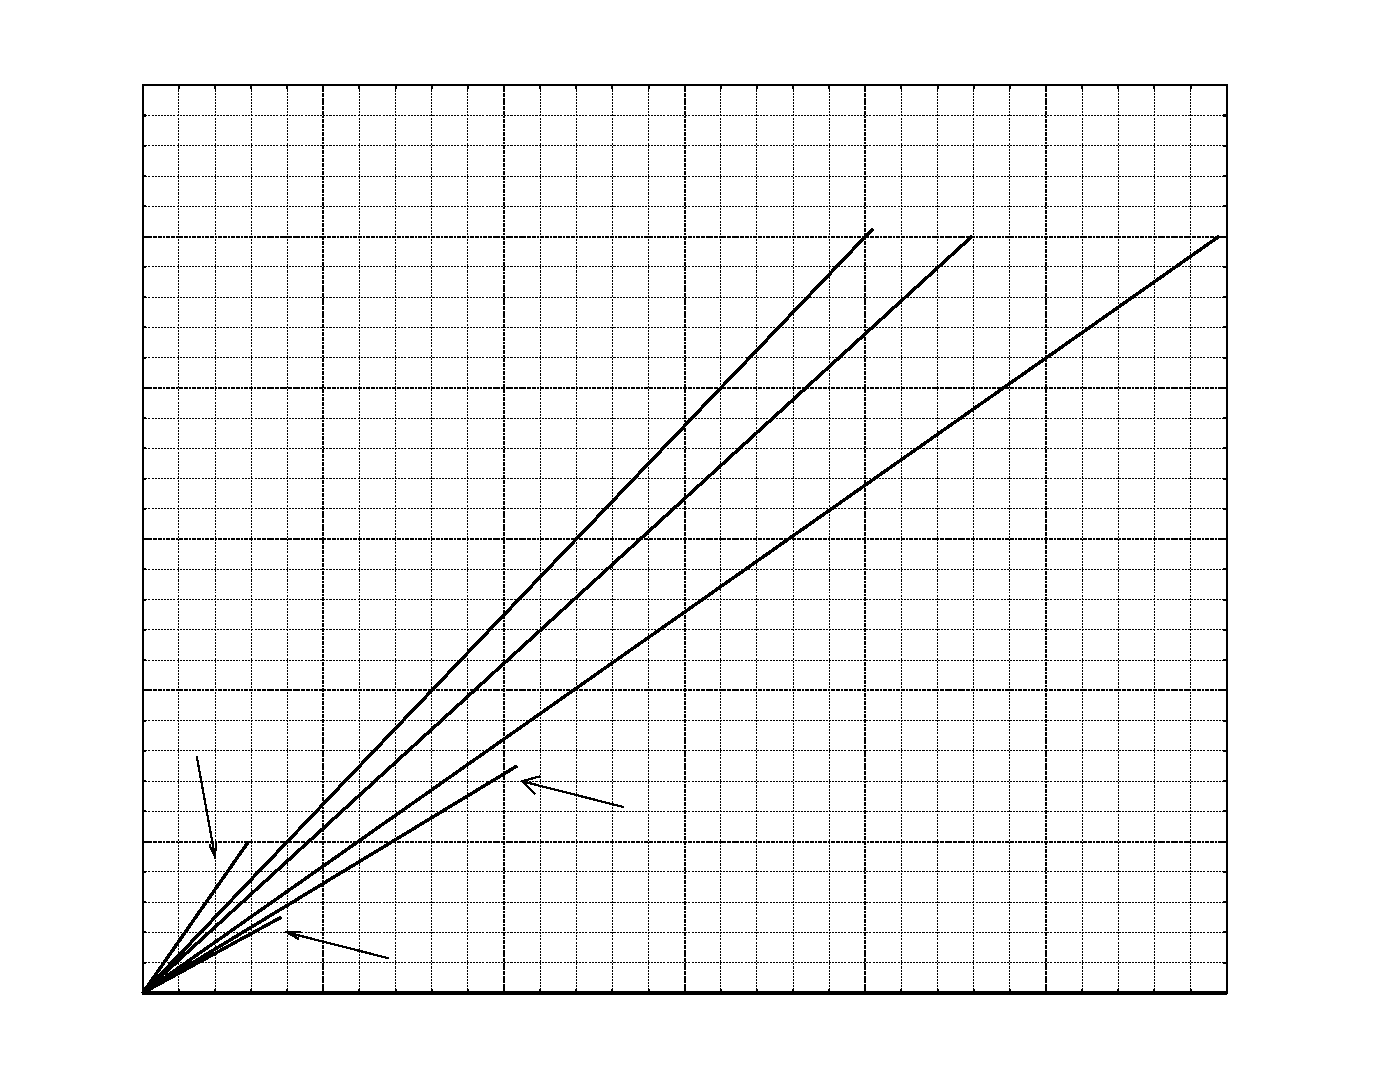
\includegraphics{../graphs/dummy}}%
    \gplfronttext
  \end{picture}%
\endgroup
